\cchapter{مروری بر ادبیات}
\label{literature}
در این بخش سعی داریم تا با مروری بر اصطلاحات و ابزارهای مورد استفاده در پژوهش‌های بررسی شده، با پیش‌نیازهای مبحث موردنظر آشنا شویم. 
\section{رایانش بدون سرور}
رایانش بدون سرور\LTRfootnote{Serverless Computing} در سال 2014 توسط شرکت آمازون برای اولین بار معرفی شد. تا قبل از این رایانش بدون سرور یک مفهوم انتزاعی \LTRfootnote{abstract} در شبکه بود که شرکت آمازون با ارائه پلتفرم \lr{AWS Lambda Functions} به معرفی آن پرداخت. سپس در سال 2016 سایر ارائه دهندگان خدمات ابری نیز به ارائه پلتفرم‌های بدون سرور خود پرداختند. در این سال به ترتیب شرکت‌های گوگل پلتفرم \lr{google cloud functions} یا به اختصار \lr{GCP}، شرکت مایکروسافت پلتفرم \lr{Microsoft Azure functions} و شرکت \lr{IBM} به معرفی \lr{IBM OpenWhisk} پرداختند. البته باید توجه داشت که مفهوم رایانش بدون سرور به طور کامل توسط ارائه دهندگاه خدمات ابری پیاده‌سازی نشده است و جای کار بسیاری دارد (با مطالعه این گزارش به مرور متوجه نواقص موجود خواهید شد).

در رایانش بدون سرور ما از نقطه قوت ماشین‌های مجازی که ایزولاسیون برنامه‌های مختلف از همدیگر بود استفاده کرده‌ایم. منتها این مورد را با مفهوم کانتینر ها پیاده‌کرده ایم. در ادامه راجع به کانتینرها نیز بحث خواهیم کرد. 

\subsection{تعریف رایانش بدون سرور}
رایانش بدون سرور مبحثی از رایانش ابری است که در آن بحث مدیریت حافظه یا \lr{Storage}، مدیریت زیرساخت و بحث‌های \lr{networking} با انتزاع بالایی به مصرف کاربر می‌رسد. به عبارت دیگر، تمامی مدیریت ای بخش‌ها بر عهده ارائه دهندگان است و ما اصلا با این بحث ها سروکاری نداریم. در واقع، هدف اصلی رایانش بدون سرور هم این است که این پیچیدگی‌ها را از کاربر بگیرد. 

به طور کلی، یک‌ پلتفرم بدون‌سرور را هر پلتفرم محاسباتی تعریف کرد که در آن مدیریت مستقیم سرور از کاربران مخفی شده و برنامه‌های کاربردی به صورت اتوماتیک در آن مقیاس‌پذیر می‌شوند و تنها هنگامی که در حال استفاده از پلتفرم هستیم، هزینه آن را پرداخت می‌کنیم. \cite{The_Rise_of_Serverless_Computing}


بسیاری از افراد، \lr{serverless} و \lr{faas} را معادل یک‌دیگر می‌دانند درحالی‌که اصلا این‌گونه نیست. در ادامه راجع به این بحث به طور مفصلی بحث خواهیم کرد اما باید بدانیم که این دو مقوله کاملا جدا از همدگیر هستند و مجددا تاکید می‌کنیم که رایانش بدون سرور یک مدل اجرایی در رایانش ابری است. 

ازطرفی رایانش بدون سرور را باید نقطه مقابل رایانش سرور آگاهانه \LTRfootnote{Server Aware} دانست که در آن از اطلاعات سرور در اختیار گرفته کاملا اگاهیم، کاملا بر مدیریت آن اشراف داریم و هرگونه تغییر از جمله متعادل‌سازی بارها، \lr{auto-scaling} و … باید توسط کاربر انجام شود.

یک مثال از پیاده‌سازی رایانش سرور آگاهانه را در زیرساخت به عنوان سرویس \LTRfootnote{Infrastructure as a service} یا به اختصار \lr{IaaS} است. در نقطه مقابل در رایانش بدون سرور هیچ کنترلی بر روی سرور نداریم، تنها می‌توانیم یک برنامه را بر روی سرور اجرا کنیم یا اجرای آن را به حالت تعلیق درآورده یا آن را از روی سرور حذف کنیم که هیچ‌کدما از این موارد نیز به صورت مستقیم انجام نمی‌گیرد؛ بلکه رابط گرافیکی و \lr{API} وجود دارد که از طریق آن‌‌ها این تغییرات را اعمال می‌کنیم. بنابراین در رایانش بدون سرور، عملا هیچ راهی برای مدیریت مستقیم سرور و زیرساخت نداریم.

شکل \ref{fig:ServerlessVSServeraware} مرز‌های بین رایانش بدون‌سرور و رایانش سرور آگاهانه را نمایش می‌دهد.  

\begin{figure}
	\centering
	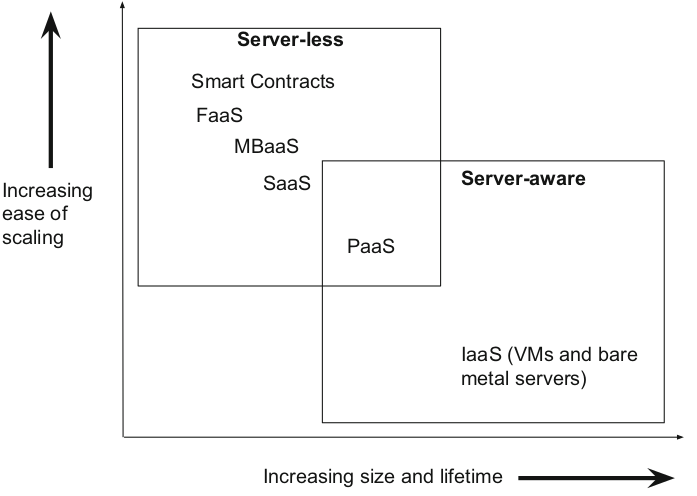
\includegraphics[width=\linewidth]{figs/ServerlessVSServeraware}
	\caption {مرز‌های رایانش بدون سرور و رایانش سرورآگاهانه}
	\label{fig:ServerlessVSServeraware}
\end{figure}

البته باید به این نکته توجه‌داشت که امروزه مرز‌های بین رایانش سرور آگاهانه با رایانش بدون سرور در حال کمرنگ شدن و بعضا از بین رفتن است و این تقسیم بندی ابدا قاطعیت ندارد.همچنین تفکیک برخی موارد مانند \lr{Platform-as-a-Serice} یا به اختصار \lr{PaaS} به راحتی انجام نمی‌گیرد بلکه این نوع رایانش می‌تواند از نوع باسرور یا بدون سرور باشد. 
در این شکل هرچه به سمت محور افقی حرکت می‌کنیم دانه‌بندی و طول‌عمر افزایش پیدا می‌کند و هرچه به سمت بالاتر می‌رویم، \lr{scaling} راحت‌تر انجام می‌گیرد. 

